% short article version of triaxial angle paper

\documentclass[main.tex]{subfiles}
%\usepackage{graphicx}

%\usepackage{geometry}
%\geometry{letterpaper, margin=1in}
%\newcounter{page}

\begin{document}


\authors{Eric Burdette}
\affiliation{1}{Department of Earth, Environmental and Planetary Sciences, Brown University, Providence, RI, USA}

\begin{keypoints}
\item High and low angle faults are less stable
\item Our results match \citet{Dieterich1992}, adding an explicitly defined compliance
\item Stiff confining media is surprisingly ineffective for stabilizing faults, while friction between pistons strongly destabilizes faults

\end{keypoints}

\doublespacing

\begin{abstract}
    The frictional stability of a confined saw-cut fault is not only a function of frictional rate parameters, but also fault angle, friction coefficient, and external forces resisting movement of the fault. We re-derive a relationship which experimentalists can use to assess stick-slip stability between different machines and experiments on the same material. As \citet{Dieterich1992a} found, very high angle and very low angle faults are theoretically less stable.
    Experimental conditions also affect stability. Confining resistance is only mildly stabilizing, while fault parallel shear resistance is strongly stabilizing. Friction between pistons is surprisingly destabilizing because it substantially increases normal stress. Low and high angle natural faults are predicted to be particularly unstable, even though they rarely rupture due to the large stresses required.
\end{abstract}



\section{Introduction}
Rock friction is an important tectonic parameter relevant for crustal strength, faulting, and earthquakes. Standard methods for studying rock friction involve pressing two blocks together with gouge material in between and controlling their shear displacement (direct shear configuration). In unconfined geometry this test is relatively simple to accomplish with square blocks and two hydraulic rams. For confined (triaxial) stress conditions present in the earth due to overlying rock, a hydrostatic pressure must be applied, which is commonly accomplished with a gas or soft solid surrounding the sample compressed in a cylindrical pressure vessel. For friction studies, two matched pistons are cut at some angle $\psi$ and pressed together with gouge in between (Figure \ref{fig:CH3_Geometry}). Shear stress is applied by increasing axial force $\sigma_1$. Confining pressure $\sigma_3$ is applied perpendicular to axial force. In this configuration there is geometric coupling between shear stress and normal stress that prevents direct use of mechanical stability relations formulated for constant normal stress. Studying geologic materials at relevant confining pressures to study earthquakes in a variety of tectonic environments requires the use of triaxial confined saw-cut piston geometry (Figure \ref{fig:CH3_Geometry}), despite its complexity. Here we present frictional stability conditions for saw-cut triaxial samples following the approach outlined by \citet{Dieterich1992a} and include cases for several common sources of experimental error.

\begin{figure}
    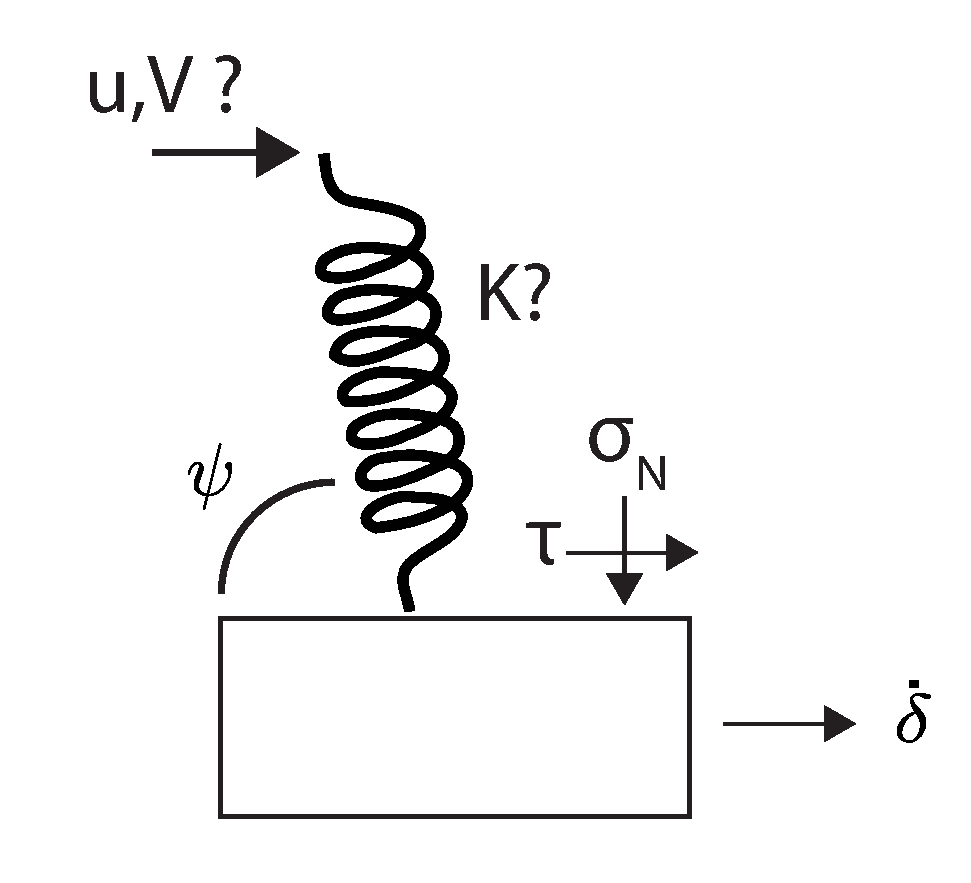
\includegraphics[width=0.25\textwidth]{Figures/D&L Stablilty High Angle Reflect.pdf}
    \caption[A high angle version of Figure 1 from \citet{Dieterich1992a}]{A modified version of the slider block and spring system from \citet{Dieterich1992a} at a high angle to illustrate the loose definition of the stiffness K. The sign convention for the angle follows \citet{karato2008deformation} for clarity. (maybe move to supplement for publication)}
    \label{fig:DL1992_highangle}
\end{figure}

\begin{figure}
    \includegraphics[width=\textwidth]{Figures/Triax_Diagram_Only.pdf}
    \caption[Geometry of triaxial displacement, stresses, and stiffness]{Geometry of a triaxially confined gouge sample between two shear pistons with a schematic spring element included to represent machine stiffness. Confining stress is labeled $\sigma_3$ and axial stress is labelled $\sigma_1$. The sign convention for the angle of the fault plane to axial stress ($\psi$) follows \citet{karato2008deformation} instead of \citet{Dieterich1992a}}
    \label{fig:CH3_Geometry}
\end{figure}

\section{Stability of Triaxial Samples}
\subsection{Standard Saw-cut Geometry}
A sample with frictional parameters $\mu_0$, A, B, and $D_c$, under confining pressure $\sigma_3$ will be stable if axial stiffness $K_{ax}$ satisfies the inequality:

\begin{equation}\label{eq:C3_1}
K_{ax,stable} \geq \frac{2}{\cos(\psi) \sin(2\psi)}\frac{\sigma_3}{1-\mu_0\tan(\psi)}\frac{(B-A)}{D_c}\frac{1}{1-\left(\mu_0-\alpha \right)\tan
(\psi)}
\end{equation}


The variables used here have the same meaning as those of \citet{Ruina1983} ($\mu_0$ is friction coefficient, A is the rate strengthening coefficient, B is rate weakening coefficient, and $D_c$ is characteristic weakening distance). This relationship shares terms with the relationship derived in \citet{Dieterich1992a}, but also explicitly describes a measurable machine stiffness $K_{ax}$ (axial stiffness), and has normal stress $\sigma_n$ in terms of measurable quantities $\sigma_3$ and $\mu_0$ (Figure \ref{fig:CH3_MainStabCompare}) The conversions are written here and the full derivation can be found in the supplement.

\begin{equation}\label{eq:C3_2}
    K_{D\&L (1992)}=\frac{d\tau}{d\delta}=\frac{d\sigma_1}{dx}\frac{\sin(2\psi)}{2}\cos{\psi}
\end{equation}

\begin{equation}\label{eq:C3_3}
    \sigma_n=\frac{\sigma_3}{1-\mu_0\tan(\psi)}
\end{equation}

Here $\tau$ is shear stress, $\sigma_n$ is normal stress, and $\delta$ is displacement on the saw-cut fault. The unstable regimes of the new relationship shares the characteristic of fault locking above angles ${\psi>arctan(\frac{1}{\mu_0})}$ (Figure \ref{fig:CH3_MainStabCompare}). In addition fault behavior becomes asymptotically unstable as fault angle ($\psi$) approaches 0. This is due to reduced shear compliance (\ref{eq:C3_1}, \ref{eq:C3_2}, \ref{eq:C3_S3}). This effect could also be important in natural settings for low angle faults.

%figure 2
\begin{figure}
    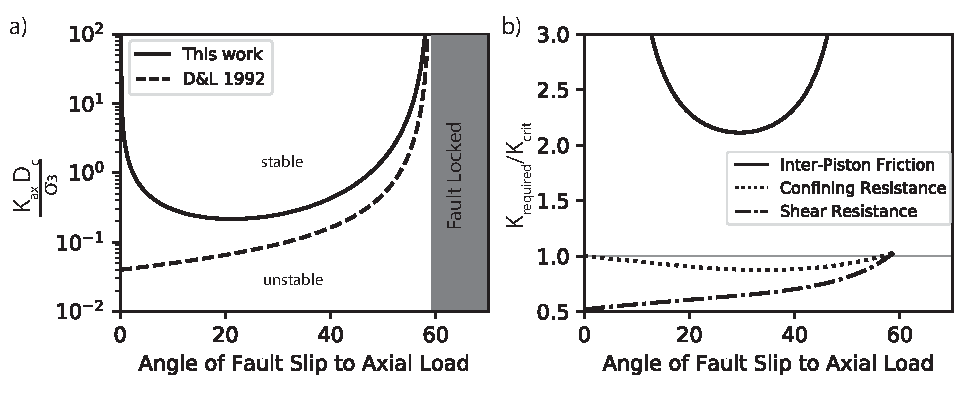
\includegraphics[width=\textwidth]{Figures/vsD&L Stablilty AngleCombo.pdf}
    \caption[Plot of critical stiffness vs. angle]{
    \textbf{a)} Plot of pressure normalized critical stiffness vs fault angle in a triaxial apparatus ($\mu_0=0.6, A=0.05, B=0.1$)
    \textbf{b)} Plot of critical stiffness of each apparatus effect relative to standard critical stiffness
    }
    \label{fig:CH3_MainStabCompare}
\end{figure}


\subsection{Effects of Inter-Piston Friction}
Frictional resistance in the direction of $\sigma_3$ will decrease sample stability by increasing fault normal stress. Cylindrical saw-cut deformation columns have an interface between an axial piston (not pictured) and the saw-cut piston so that the saw-cut piston can move normal to $\sigma_1$. If this interface were frictionless it would not affect results, but it has some resistance in practice. The piston interface friction $\mu_r$, which is always normal to $\sigma_1$ can be simply added to the confining resistance as:
\begin{equation}\label{eq:C3_4}
    \sigma_3'=\sigma_3+\mu_r\sigma_1
\end{equation}
When this is used in the derivation it results in both changes in steady state normal stress as well as the stiffness inequality:
\begin{equation}\label{eq:C3_5}
    \sigma_{n,ss}=\frac{\sigma_3}{1-\mu_r-\mu_0\left(\mu_r\cot (\psi)+\tan(\psi)\right)}
\end{equation}
\begin{equation}\label{eq:C3_6}
    K_{ ax} \geq \frac{2}{\cos(\psi)}\sigma_{n,ss}\frac{(B-A)}{D_c}\frac{1}{\left(1-\mu_r\right)\sin(2\psi)-\left(\mu_0-\alpha \right)\left(1-\cos
    (2\psi)+\mu_r(1+\cos(2\psi))\right)}
\end{equation}
Both of these quantities are greater (less stable) than their standard counterparts and a friction coefficient of 0.1 will double required axial stiffness for 30 degree faults (Figure \ref{fig:CH3_MainStabCompare}).

\subsection{Effect of Confining Resistance}
Some triaxial apparatuses use weak solids around their samples. The weak solids present resistance to piston expansion normal to axial stress. This can be easily represented by adding a linear viscosity to $\sigma_3$ :
\begin{equation}\label{eq:C3_7}
    \sigma_3'=\sigma_3+\eta\dot{\delta}\sin(\psi)
\end{equation}
This can be used to derive the stability inequality:
\begin{equation}\label{eq:C3_8}
    \sigma_{n,ss}=\frac{\sigma_3+\eta \dot{\delta}_{ss} \sin(\psi)}
    {1-\mu_0\tan(\psi)}
\end{equation}

\begin{equation}\label{eq:C3_9}
K_{ax} \geq 
\frac{1}{\cos(\psi)\sin(2\psi)}\frac{1}{(1-(\mu_0-\alpha)\tan(\psi))}
\frac{1}{D_c}
\left(2\sigma_{n,ss}(B-A) -\mu_0\eta\dot{\delta}_{ss}\sin(\psi)(1+\sin(2\psi)+\cos(2\psi))\right)
\end{equation}
The resulting stability inequality has higher normal stress, but also terms resisting high speed fault movement, which have opposing effects on stability (Table \ref{tab:CH3_stabilitytable}). In most cases confining resistance does not substantially affect fault stability (Figure \ref{fig:CH3_MainStabCompare}).

\subsection{Effect of Shear Drag}
Most triaxial pistons are covered in rubber or metal jackets whose resistance can easily be represented by a linear viscous term ($\eta\dot{\delta}$) added to shear stress. The effect opposes velocity weakening and stabilizes faults.
\begin{equation}\label{eq:C3_10}
\sigma_{n,ss}=\frac{\sigma_3+\eta  \dot{\delta}_{ss}\tan(\psi)}{1-\mu_0\tan(\psi)}
\end{equation}
\begin{equation}\label{eq:C3_11}
K_{ ax} \geq \frac{1}{\cos(\psi)\sin(2\psi)}\frac{1}{1-(\mu_0-\alpha)\tan(\psi)}\frac{1}{D_c}\left(2\sigma_{n,ss}(B-A) -2\eta \dot{\delta}_{ss}\right)
\end{equation}
The stabilization provided by viscous strengthening can be very strong and is especially effective on shallow faults due to their low shear stresses (Figure \ref{fig:CH3_MainStabCompare}).



\section{Piston Offset Stiffness Effects}
The triaxial piston geometry has a significant limitation in that area of contact changes during slip. This causes stress for a given force to increase ($\tau_fault$, equation \ref{eq:C3_15}) on the effective fault which also changes effective stiffness to decrease. To illustrate this we switch displacement to a general fractional shear length s ($\frac{slip}{\text{fault length}}$) and consider fault shear stress $\tau$:
\begin{equation} \label{eq:C3_12}
    s(\delta)=\frac{\delta}{d_0/\sin{\psi}}
\end{equation}
\begin{equation} \label{eq:C3_13}
    f(s) = \frac{\text{Area}}{\text{Area}_0}= 1 - 1.2082 {s} - 0.19134 {s}^2 + 0.39461 {s}^3
\end{equation}
where piston diameter is $d_0$. $f(s)$ is a polynomial less than 1 for slip s from 0 to 1. We can define the spring portion of a block-slider system in terms of fractional slip:
\begin{equation} \label{eq:C3_14}
    \tau_{\sigma_1}(s)=\tau_{\sigma_1, ss}-K_{{d\tau}_{\sigma_1},ds}*(s-s_{ss})
\end{equation}
where $\tau_{\sigma_1}$ is shear stress calculated from applied load and geometry, ss denotes steady-state, and stiffness $K_{{d\tau}_{\sigma_1},ds}$ is defined in terms of axial/geometric quantities that do not change with slip (see supplement). The affect of area change can then be accounted for:
\begin{equation} \label{eq:C3_15}
    \tau_{fault}=\tau_{sigma_1}(s)/f(s)
\end{equation}
where $\tau_{fault}$ is shear stress on the portion of the fault in contact.  We are interested in the fault properties so we need to substitute eq. \ref{eq:C3_14} into \ref{eq:C3_15}, and then differentiate with respect to s using the product rule which yields:
\begin{equation} \label{eq:C3_16}
    \frac{d\tau_{fault}}{ds}(s)=\tau_{\sigma_1}(s)*\frac{-1}{f^2}\frac{df}{ds}-K_{\tau,s}/f(s)
\end{equation}

The two resulting terms for effective slip stiffness counteract each other. They also always have different polynomial orders which allows the possibility of transitional stability.

The most important effect to note is that steady-state shear stress controls the first term in equation (\ref{eq:C3_16}). If starting load is too high, effective stress will only increase during unloading and the fault will always be unstable (Figure \ref{fig:CH3_Offset_plots}).

%figure 3
\begin{figure}
    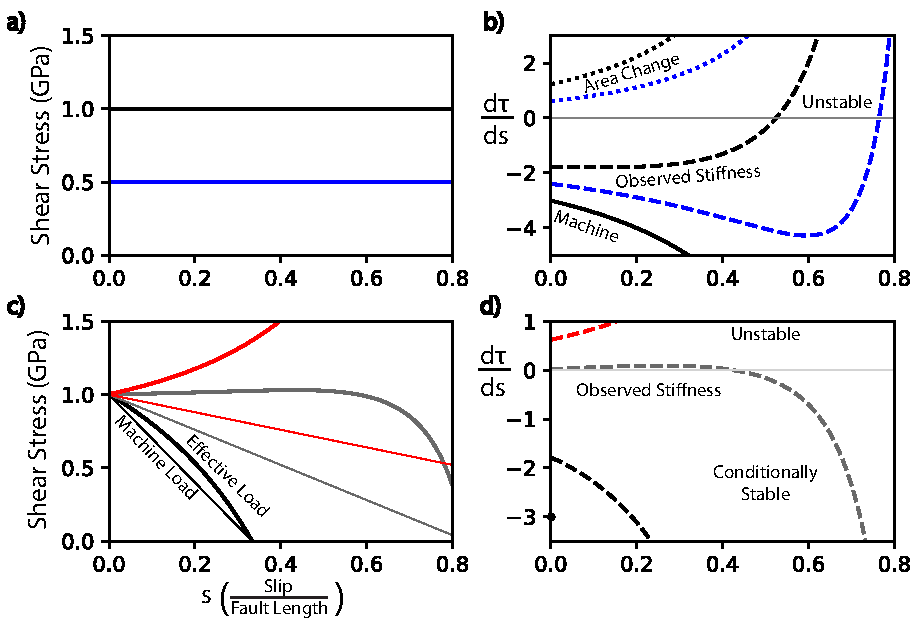
\includegraphics[width=0.75\textwidth]{Figures/AreaOffsetStability_conststress_relax-mod.pdf}
    \caption[Area offset effects on triaxial stability]{
    \textbf{a)} Constant applied shear stress at two levels vs s ($K_{\tau,s}=3$)
    \textbf{b)} Resulting shear stress derivatives split into area reduction contribution (dotted), machine stiffness change (solid), and the resulting instantaneous combined stiffness (dashed)
    \textbf{c)} Relaxation shear stress vs s (machine=thin, area corrected=thick) for three different machine stiffnesses (3 GPa/mm (black), 1.2 GPa/mm (grey), and 0.6 GPa/mm (red)) on a quarter inch diameter sample with a 45 degree fault.
    \textbf{d)} Relaxation area corrected instantaneous stiffness vs s.
    }
    \label{fig:CH3_Offset_plots}
\end{figure}

\section{Implications}
\subsection{Laboratory Implications}
Observing instability in the laboratory is important for understanding earthquake phenomena. Accuracy in measurements is critical for extrapolating the observed data to the earth so the derived relationships should be incorporated into stability assessments. A few rules of thumb are substantiated here: stiff machines prevent instability and stability determination is most accurate at low fault displacement. A few new rules should be considered: friction between axial and shear pistons should be minimized, and low fault angles may be unexpectedly unstable. A summary of each of the external experimental effects on stability is presented in the table below.

\begin{table}
\caption[Table of triaxial experimental influences' effects on normal stress and velocity dependence of rate-state friction faults]{Experimental influences on stability.}
\label{tab:CH3_stabilitytable}
 \begin{tabular}{||c | c | c | c||} 

 \hline
 Effect Type & Stability? & Normal Stress & Velocity Dependence \\ [0.75ex] 
 \hline\hline
 Inter-Piston Friction & Less Stable & Increases & No Change \\ [0.5ex] 
 \hline
 Confining Resistance & More Stable & Increases & Rate Strengthens \\[0.5ex] 
 \hline
 Shear Resistance & More Stable & No Change & Rate Strengthens \\ [0.5ex] 
 \hline
\end{tabular}
\end{table}


\subsection{Natural Implications}
Low angle normal faults are a tempting candidate to apply the stability calculations derived here, but we can only address one portion of the puzzle: propensity for dynamic rupture (earthquakes). If a fault is described as a thin elastic sheet as in \citet{forsyth1992finite} then the derived relationship would hold and low angle faults would be substantially less stable. In natural faults low angle portions of the fault tend to be near the brittle-ductile transition (cite) where no seismicity would be expected, but the instability of low fault angles could cause ruptures to propagate deep into the crust generating large earthquakes (mentioned briefly in \citet{wernicke1995low}). 
[obviously a weakening mechanism is needed, but their response amplitudes are all controlled by stiffness and therefore angle. We could point to thermal pressurization or silica gel weakening]

Reverse faults are similar to the laboratory setup and should be very unstable at steep dip angles close to the frictional lock-up. The relationships derived above would hold for the low coefficients of friction required for steeply dipping faults to fail and rupture. It is possible the frictional instability explains the secondary peak at high dip observed in compilations of large magnitude reverse fault earthquakes \citep{sibson1998dip}. 

Some elusive aspects of strike-slip faults could be be explained if their stiffness can be simplified into a representation parallel to their compression axis. The San Andreas fault provides one example where some fault segments trend in anomalous P-shear directions \citep{moore1991comparative}. All the off-strike fault traces would be more unstable because they are at high and low angles to the predominantly N-S compression. N-leaning segments would tend to be less affected because of the asymmetry of the stability curve, while W-leaning segments could be strongly affected as they are closer to the high-normal stress lock-up angle. Mineralogy of the area is known to be complex with weak anisotropic clays \citep{lockner2011low}, so instability is unlikely to be the only cause for the existence of W-leaning segments.
 

%figure 4
\begin{figure}
    \includegraphics[width=0.4\textwidth]{Figures/Sibson-Xie1998F3.png}
    \caption[Fault Angle vs. number for surveyed faults]{Fault Angle vs. number for surveyed faults. Reproduced from \citet{sibson1998dip}.
    }
    \label{fig:CH3_NaturalData}
\end{figure}



\section{Conclusions}
\begin{enumerate}
    \item Confined saw-cut fault stability is not only a function of frictional rate parameters, but also fault angle, friction coefficient, and external forces resisting movement of the fault.
    \item We derive a relationship which experimentalists can use to assess stick-slip stability between different machines and experiments on the same material.
    \item Very high angle and very low angle faults are theoretically less stable.
    \item Experimental conditions affect stability. Confining resistance is only mildly stabilizing, while fault parallel shear resistance is strongly stabilizing. Friction between pistons is surprisingly destabilizing because it substantially increases normal stress.
    \item Low and high angle natural faults are predicted to be unusually unstable, even though they rarely rupture due to the large stresses required.
\end{enumerate}

\acknowledgments
 I would like to thank Jim Dieterich for kindly providing his notes from the original derivation.

\clearpage

\subfile{./EB_RSTriax_NormalStress_Derivation.tex}
\subfile{./EB_RSTriax_Full_Derivation.tex}

\clearpage

\singlespacing
% \bibliographystyle{apalike}
% \bibliography{Feb19_refs_2.bib}


\end{document}